
%%%%%%%%%%%%%%%%%%%%%%% file typeinst.tex %%%%%%%%%%%%%%%%%%%%%%%%%
%
% This is the LaTeX source for the instructions to authors using
% the LaTeX document class 'llncs.cls' for contributions to
% the Lecture Notes in Computer Sciences series.
% http://www.springer.com/lncs       Springer Heidelberg 2006/05/04
%
% It may be used as a template for your own input - copy it
% to a new file with a new name and use it as the basis
% for your article.
%
% NB: the document class 'llncs' has its own and detailed documentation, see
% ftp://ftp.springer.de/data/pubftp/pub/tex/latex/llncs/latex2e/llncsdoc.pdf
%
%%%%%%%%%%%%%%%%%%%%%%%%%%%%%%%%%%%%%%%%%%%%%%%%%%%%%%%%%%%%%%%%%%%


\documentclass[runningheads,a4paper]{llncs}

\setcounter{tocdepth}{3}
\usepackage{graphicx}
\usepackage{booktabs}
\usepackage{times}
\usepackage{epsfig}
\usepackage{amsmath}
\usepackage{amssymb}
\usepackage{multirow}

\usepackage{url}
\urldef{\mailsa}\path|{alfred.hofmann, ursula.barth, ingrid.haas, frank.holzwarth,|
\urldef{\mailsb}\path|anna.kramer, leonie.kunz, christine.reiss, nicole.sator,|
\urldef{\mailsc}\path|erika.siebert-cole, peter.strasser, lncs}@springer.com|
\newcommand{\keywords}[1]{\par\addvspace\baselineskip
\noindent\keywordname\enspace\ignorespaces#1}

% macros for referencing figures, tables, equations and sections
\def\figpath{./figs}
\newcommand{\fref}[1]{Figure~\ref{#1}}
\newcommand{\eref}[1]{(\ref{#1})}
\newcommand{\tref}[1]{Table~\ref{#1}}
\newcommand{\sref}[1]{Section~\ref{#1}}
\newcommand{\aref}[1]{Algorithm~\ref{#1}}

% alternatives if booktabs not available
%\newcommand{\toprule}{\hline\noalign{\smallskip}}
%\newcommand{\midrule}[1]{\cline{#1}\noalign{\smallskip}}
%\newcommand{\bottomrule}{\hline\noalign{\smallskip}}

% maths macros
\def\G{G}
\def\Gx{G_x}
\def\Gy{G_y}
\def\Gxx{G_{xx}}
\def\Gxy{G_{xy}} \def\Gyx{G_{yx}}
\def\Gyy{G_{yy}}
\def\Ix{I_x}
\def\Iy{I_y}
\def\Ixsqr{I_{x^2}}
\def\Iysqr{I_{y^2}}
\def\Ixx{I_{xx}}
\def\Ixy{I_{xy}}
\def\Iyy{I_{yy}}
\def\dtcwt{DT-$\mathbb{C}$WT}
\def\figpath{./figs}
\def\ie{i.e.}
\def\eg{e.g.}
\def\etal{\emph{et al.}}

% command for adding inline comment to text
\newcommand{\comment}[1]{}

\begin{document}

\mainmatter  % start of an individual contribution

% first the title is needed
\title{Segmenting and Estimating the Orientation of Retinal Vessels using Random Forests}

% a short form should be given in case it is too long for the running head
\titlerunning{Segmenting and Estimating the Orientation of Retinal Vessels}

% the name(s) of the author(s) follow(s) next
%
% NB: Chinese authors should write their first names(s) in front of
% their surnames. This ensures that the names appear correctly in
% the running heads and the author index.
%
\author{*}%
%\thanks{Please note that the LNCS Editorial assumes that all authors have used
%the western naming convention, with given names preceding surnames. This determines
%the structure of the names in the running heads and the author index.}%
%\and Ursula Barth\and Ingrid Haas\and Frank Holzwarth\and\\
%Anna Kramer\and Leonie Kunz\and Christine Rei\ss\and\\
%Nicole Sator\and Erika Siebert-Cole\and Peter Stra\ss er}
%
%\authorrunning{Lecture Notes in Computer Science: Authors' Instructions}
% (feature abused for this document to repeat the title also on left hand pages)

% the affiliations are given next; don't give your e-mail address
% unless you accept that it will be published
\institute{*}
%Tiergartenstr. 17, 69121 Heidelberg, Germany\\
%\mailsa\\
%\mailsb\\
%\mailsc\\
%\url{http://www.springer.com/lncs}}

%
% NB: a more complex sample for affiliations and the mapping to the
% corresponding authors can be found in the file "llncs.dem"
% (search for the string "\mainmatter" where a contribution starts).
% "llncs.dem" accompanies the document class "llncs.cls".
%

\toctitle{Lecture Notes in Computer Science}
\tocauthor{ }
\maketitle


\begin{abstract}
Segmenting image structure whilst also estimating its orientation underpins applications including retinography, digital mammography, fingerprint analysis and many more. We compare filter banks composed of second derivatives and the Dual Tree Complex Wavelet Transform (\dtcwt) as a means for representing local image structure, then investigate how Random Forest classifiers and regressors can use the responses to these filter banks in order to segment and predict the orientation of image structure. For a quantitative evaluation, we use the publicly available DRIVE database of retinal images, producing segmentation results that match the state-of-art ($A_z = 0.962$) whilst estimating orientation with superior accuracy to standard analytical methods.
%\keywords{We would like to encourage you to list your keywords within the abstract section}
\end{abstract}

\section{Introduction}
\label{s:introduction}
Segmenting curvilinear structures such as blood vessels, ducts and nerve fibres in medical images is an important task, as shown by the extensive literature in the field~\cite{Papari_Petkov_IVC11,Staal_etal_TMI04,Ricci_Perfetti_TMI07}. In retinography, for example, a map of vessel structure helps us to ignore vessels when counting microaneurysms or to detect newly formed vessels (neovascularisation), and therefore better quantify progression in diseases such as diabetic retinopathy.

Similarly, estimating the local \emph{orientation} of curvilinear structure is also important, though the literature in this area is more limited~\cite{Freeman_Adelson_TPAMI91,Koenderink_vanDoorn_TPAMI92}. At a low and intermediate level, knowing the orientation of curvilinear linear structure is important for steering computation~\cite{Sonka_99}, extracting profiles~\cite{Staal_etal_TMI04}, grouping and tracking curvilinear features~\cite{Aylward_Bullitt_TMI02}, and directional filtering such as nonmaximal suppression and anisotropic smoothing.

Applications requiring higher level interpretation are more diverse. Again, in retinography (\fref{f:retinography}) the rate of change of orientation (\ie~tortuosity) of blood vessels can serve as a diagnostic indicator of vascular disease~\cite{Hart_etal_IJMI99}. In x-ray mammography, local orientation can be used to detect the patterns of radiating curvilinear structures (known as spicules) that are often associated with malignant lesions~\cite{Karssemeijer_teBrake_TMI96}.
%
\begin{figure}[t]
\centering
\begin{tabular}{@{}c c c c@{}}
\includegraphics[width=0.24\columnwidth]{\figpath/retina/02_test} &
\includegraphics[width=0.24\columnwidth]{\figpath/retina/02_manual1_pos} &
\includegraphics[width=0.24\columnwidth]{\figpath/retina/02_segmentation} &
\includegraphics[width=0.24\columnwidth]{\figpath/retina/002_orientation_mag} \\
(a) & (b) & (c) & (d)\\
\noalign{\smallskip}
\end{tabular}
%
\caption{Estimating orientation in retinography: %
(a) input image; %
(b) ground truth mask indicating pixels belonging to a vessel; %
(c,d) vessel segmentation and orientation estimation using random forests and \dtcwt{} features. In (d), hue and brightness indicate the angle and magnitude of the predicted orientation vector. %
}
\label{f:retinography}
\end{figure}
%

In this paper we focus on segmenting vessels and estimating their orientation in retinograms, and we provide the results of extensive evaluation using the publicly available DRIVE dataset~\cite{Staal_etal_TMI04}. However, our methods -- using a filter bank to describe local structure, and combining responses with a suitable classifier or regressor -- are generally applicable for working with linear structures in any image type where ground truth is available, and may be extended to 3D if necessary.

%Our main contributions are threefold.
We thus make three main contributions: first, we present state-of-the-art segmentation results that combine random forest classification with \dtcwt{} image features.
Second, we review the basic theory on estimating orientation and show that using a regression approach to combine filter responses across all scales and orientations gives significantly better estimation accuracy compared to combining analytically the responses from the scale at which the total magnitude of response is greatest. With regard to this, we note that the use orientation in this setting has only briefly been explored~\cite{Berks_etal_IPMI11} with the vast majority of previous work using an analytical approach. As such we provide the technical details of orientation regression in random forests and provide a comprehensive evaluation of different combinations of filter-bank and analytic/regression methods. Lastly, we show that the magnitude orientation predicted from the regression forests contain information potentially useful for further processing and analysis.
%
\section{Choosing an Image Filter Bank}
\label{s:filters}
Directional first and second second derivatives of Gaussian kernels, typically applied at multiple scales, are widely used for detecting and estimating the orientation of linear structures such as edges and ridges (\ie,~symmetric, bar-like structures). They have the advantage of being both separable (and thus efficient to compute) and steerable (\ie~the response to a filter at an arbitrary angle can be computed from a fixed number of bases).

% One filter bad...
An orthogonal pair of first derivative kernels, with odd symmetry, can estimate edge orientation and the associated response at that angle. This fails, however, when applied at the centre of a ridge (such as a vessel) because both responses are close to zero and the orientation cannot be reliably computed. Second derivatives are therefore a better choice when working with vessels and are included in our experiments as a baseline performance comparison. Again, three separable basis filters -- $\Gxx$, $\Gyy$ and $\Gxy$ (\fref{f:filters}a,b) -- give the orientation and corresponding steered response~\cite{Freeman_Adelson_TPAMI91,Koenderink_vanDoorn_TPAMI92,Karssemeijer_teBrake_TMI96}:
%
\begin{equation}
\theta = \frac{1}{2}\tan^{-1}\left[ \frac{2\Ixy}{\Ixx-\Iyy} \right], \,\,\,\, R(\theta) = \Ixx \cos^2(\theta) + \Iyy \sin^2(\theta) + \Ixy \sin(2\theta)
\label{e:r2s}
\end{equation}
%
\noindent where $\Ixx$, $\Iyy$ and $\Ixy$  are the image responses to the respective filters $\Gxx$ etc. Solving for $\theta$ yields two perpendicular solutions corresponding to the maxima and minima of~\eref{e:r2s}, and thus the steered response to both must be checked to determine the correct solution.\footnote{This solution is a mathematical reworking of orientation estimation through Hessian filtering~\cite{Frangi_MICCAI98,Sato_MIA98} in which a Hessian matrix is filled with the $\Ixx$ and $\Iyy$ on the leading diagonal and $\Ixy$ terms on the off diagonal. Decomposing this matrix produces eigenvectors with direction $\theta$ and $\theta^{\perp}$ associated with eigenvalues $R(\theta)$ and $R(\theta^{\perp})$.} Conversely, however, second derivatives fail at edges where the responses of an odd image feature to an even filter are close to zero.

% ...two filters good
Intuitively, using both odd and even filters should be most flexible for the complete range of image structures. More formally, we seek a Hilbert pair of filters that are $90^\circ$ out of phase. In addition to providing a consistent measure of orientation for all structure types, the relationship between the paired responses (\ie~the local phase) provides a measure of symmetry in a profile of the structure perpendicular to its orientation that could be used to discriminate between vessels and other background structures, and thus may be advantageous for segmentation.

Unfortunately, the Hilbert pair of a directional Gaussian second derivative cannot be computed analytically, and whilst a discrete approximation exists~\cite{Freeman_Adelson_TPAMI91} such pairs have not often been used in practice. Gabor filters (combining both sine and cosine functions with a Gaussian kernel) are a more popular choice~\cite{Daugman_TASSP88} but these are neither steerable nor separable; the cost of computing and storing the responses at multiple orientations and scales therefore makes them impractical for large images.
%
\begin{figure}[t]
\centering
\begin{tabular}{@{}c c c c@{}} % @{} removes padding around the edge of the table
\includegraphics[width=0.2\columnwidth]{\figpath/Gxx} &
\includegraphics[width=0.2\columnwidth]{\figpath/Gxy} &
\includegraphics[width=0.2\columnwidth]{\figpath/dt_cwt_r4} &
\includegraphics[width=0.2\columnwidth]{\figpath/dt_cwt_c4} \\
(a) & (b) & (c) & (d)\\
\noalign{\smallskip}
\end{tabular}
%
\caption{(a,b)~Second derivatives, $\Gxx = \Gyy^T$ and $\Gxy$; (c,d)~Real and complex responses of the \dtcwt{} $15^\circ$ subband.}
\label{f:filters}
\end{figure}

To overcome these problems, we use the Dual-Tree Complex Wavelet Transform (\dtcwt{}~\cite{Kingsbury_PTRSLA99}) that uses decimation and separable filters for efficiency while still producing approximately shift-invariant coefficients. Though the construction of the \dtcwt{} is beyond the scope of this paper, here it suffices to know that at every scale the transform generates a complex response at six angles (approximately $\pm15^\circ$, $\pm45^\circ$ and $\pm75^\circ$), where the real and imaginary parts are the responses to a pair of filters that are $90^\circ$ apart in phase (\fref{f:filters}c,d). This decomposition has redundancy of just 4:1 making it practical to store the decomposition of even large images such as mammograms. The decimated coefficients can then be interpolated at any spatial location (\eg~at points on the original pixel grid). By computing phase differences both spatially and across scale is possible to analytically compute local orientation~\cite{Anderson_ICP05}. Alternatively, the coefficients may be passed directly into a suitably trained regressor to estimate orientation~\cite{Berks_etal_IPMI11} and this is the approach we explore further in this work.

\section{Segmentation via Classification, Orientation via Regression}
\label{s:learning}
% Regressing orientation
Segmenting vessels by training a classifier to label individual pixels as either structure or background is a natural approach that has provided previous state-of-the-art results for retinal data~\cite{Staal_etal_TMI04}. By labelling the ground truth with orientation we can also train a regressor to predict orientation from the same features used during segmentation, presenting three clear benefits: orientation can be estimated even where an analytic solution is not obvious (as in the \dtcwt{}); pooling responses over scales and in a local neighbourhoods is straightforward; and it is easy to account for factors such as non-Gaussian noise in medical images and an arbitrary distribution over line widths.

% Random Forest regression (in general)
As our task requires a model that can learn complex nonlinear relationships over large numbers of variables (with absolute scales that are incommensurate) at a reasonable computational cost, Random Forests~\cite{Breiman_ML01} are well suited to our tasks. A forest consists of $N$ binary classification or regression trees, each of which is built using an independent sample of the training data to reduce correlation between trees; for small datasets this is done via bootstrapping, though large datasets can simply be sampled without replacement. To reduce correlation between trees further, each tree node uses only a random subset of the possible feature dimensions.

% Specific to our problem
\subsection{Predicting Orientation via Random Forests}
Using a Random Forest to predict accurate orientations in retinograms demands a careful design that has not previously been addressed, and this is one contribution of our work.

First, we note that the only comparable study of which we are aware~\cite{Berks_etal_IPMI11} used orientation angle as the output to be predicted, which does not permit correct treatment due to wraparound (orientations may be classed as far apart when they are, in fact, close together). Instead, we define an ideal orientation (\eg~from ground truth data) by a unit vector in the complex plane, $t_k = \cos 2\theta_k + i\sin 2\theta_k$, where doubling the angle makes orientation invariant to direction~\cite{Mardia_Jupp_00}.

Defining orientations in this way also permits a correct definition of variance, the angular dispersion~\cite{Mardia_Jupp_00}, that is defined as the magnitude of the mean vector over the sample set \ie~$D = |(\sum{t_k})/N|$. This has a maximum of 1 when all $t_k$ are equal, and a minimum of 0 when orientations are distributed uniformly about the circle or when the sample consists of pairs exactly $180^\circ$ apart. Since the dimension and threshold that define each split in a regression tree are typically chosen to maximise the sum of the variances of the two samples produced by the split, this correct measure ensures better splits within the tree structure and more accurate regression.

When choosing the depth of the tree, we have found (as have others~\cite{Criminisi_MICCAI11}) that rather than constructing trees until completely pure leaves are found (\ie~nodes with $D$ arbitrarily close to 1), it is both more efficient and more robust to stop when some minimum leaf size is reached (typically 0.05\% of the total input samples). We then store the mean sample vector of orientations at each leaf, in effect encoding a summary of the sample of orientations at that point in the feature space. The magnitude of these vectors can be viewed as the confidence in a leaf's ability to predict orientation.

When we apply the regression forest to predict orientations, we take the mean of the prediction vectors from the individual trees. Thus trees which described the input feature poorly (and so return a leaf orientation vector with small magnitude) contribute little to the overall orientation prediction, relative to trees that were able to match the input feature to a pure sample of orientations. Implementing forests in this way produces orientation predictions that are both more accurate and more robust (\ie~resistant to overtraining) than those from unpruned trees with uniform weighting of leaf orientations. Moreover we propose that the final prediction (which can be viewed as measure of forest's confidence in the estimated orientation) provides useful information for further processing.

In the context of predicting orientation in retinograms, we must also deal with the boundary effects caused by the strong edge of the camera aperture. Given enough training examples, however, a forest should be able to learn the difference between spurious responses and genuine structure. We therefore sample at least 10\% of the points for each tree from a radial region within 32 pixels of the edge (the approximate half-width of largest filter supports).
%\footnote{A more principled manner of overcoming such misclassifications could be the IPMI paper from last year~\cite{}, warrants further investigation}

\section{Experiments}
\label{s:expts}
The publicly available DRIVE dataset~\cite{Staal_etal_TMI04} contains 40 full colour retinogram images (\fref{f:retinography}a) of $565{\times}584$ pixels, split into 20 training and 20 test images. A hand-labelled mask that indicates vessel pixels (\fref{f:retinography}b) is also available for every image, providing ground truth for vessel segmentation via classification. We compute ground truth orientation, $t_{gt} = \cos 2\theta_{gt} + i\sin 2\theta_{gt}$, at the vessel centres by skeletonising the masks and computing a locally linear fit; we then assign to every vessel pixel the orientation of its nearest centreline pixel.
%
\comment{Why 200k points? Was this limit dictated by system requirements?}

For training, we first transformed all images to monochrome via a weighted sum of the three RGB channels (this proved marginally more successful than extracting features from all or any of the channels individually) and computed their \dtcwt{}. We generated a classification forest of 200 trees, for each of which we randomly selected 100\,000 vessel and 100\,000 background pixels from the training images and extracted a feature vector of the \dtcwt{}  responses across all six sub-bands (\ie~basis filter orientations) at the first five scales in a $3{\times}3$ neighbourhood about each pixel. For orientation regression, we repeated the process but using only the vessel pixels (as we do not define the orientation of background pixels in this work).

To provide a baseline comparison for orientation estimation we filtered the images with Gaussian derivatives $\Gxx$, $\Gyy$ and $\Gxy$ at scales of $\sigma{=}[0.5, 1, 2, 4, 8]$ and solved~\eref{e:r2s} to determine analytically the orientation that maximised the response over all scales. To quantify any gain when using learning over an analytic solution, we also trained classification and regression forests as above but using feature vectors composed of the $\Gxx$, $\Gyy$ and $\Gxy$ responses.

Finally, to verify that useful information could be learned from the non-linear relationships in the \dtcwt{} responses, we trained a linear regressor to predict orientation from a single set of randomly sampled 100\,000 vessel pixels.

To test segmentation, we applied each classifier to determine the vessel probability at every pixel for every test image (\fref{f:retinography}c). We then computed the ROC curve and used the area under the curve, $A_z$, as a single measure of performance (\tref{t:retinopathy}). Both forest classification methods achieved an $A_z$ exceeding what is recognised as the current state-of-the-art~\cite{Staal_etal_TMI04} although, slightly surprisingly, the Gaussian derivative filter proved more successful than the \dtcwt{}.
%
\begin{table}[tb]
\centering
%\small
\input{retinogram_table.txt}
%
\caption{Classification performance, defined by the area under the Receiver Operating Characteristic (ROC) curve, $A_z$, and median absolute error (MAE) over orientation, expressed in degrees for test images 01-20 of the DRIVE retinogram database. Results are shown both for all pixels within the vessel and (in brackets) only those pixels along the centre of the vessel.}
\label{t:retinopathy}
\end{table}
%

For orientation, we estimated the complex output, $t_{est} = \cos 2\theta_{est} + i\sin 2\theta_{est}$, using each regressor in turn and computed the error with respect to ground truth,
%
\begin{equation}
	\theta_{err} = \frac{1}{2}|\angle(t_{gt} \cdot t_{est}^*)|,
\end{equation}
%
\noindent at labelled vessel pixels in the test image, where $t^*$ denotes the complex conjugate of $t$. When comparing the performance of different features and regressors, we generated the cumulative distribution function over error (\fref{f:retina_graphs}a) and summarised performance by the median\footnote{The median is more robust than the mean to outliers in the error distribution.} errors over both the whole vessel and over the centre line only (\tref{t:retinopathy}). Furthermore, because faint and narrow vessels are the most challenging (and potentially interesting) it is worth quantifying how well each method performs for vessels of different sizes and contrasts (\fref{f:retina_graphs}b,c). To do so, we estimated vessel width using the distance transform of the vessel mask, and defined line contrast as the absolute difference between the vessel intensity and the mean intensity of background pixels in a $15{\times}15$ neighbourhood.
%
\begin{figure}[t]
\centering
\def\figwidth{0.36\textwidth}
\begin{tabular}{@{}c c@{}}
\includegraphics[width=\figwidth]{\figpath/retina/cumfreq} &
\includegraphics[width=\figwidth]{\figpath/retina/thickness_vs_error-summ} \\
(a) & (b)\\
\includegraphics[width=\figwidth]{\figpath/retina/contrast_vs_error-summ} &
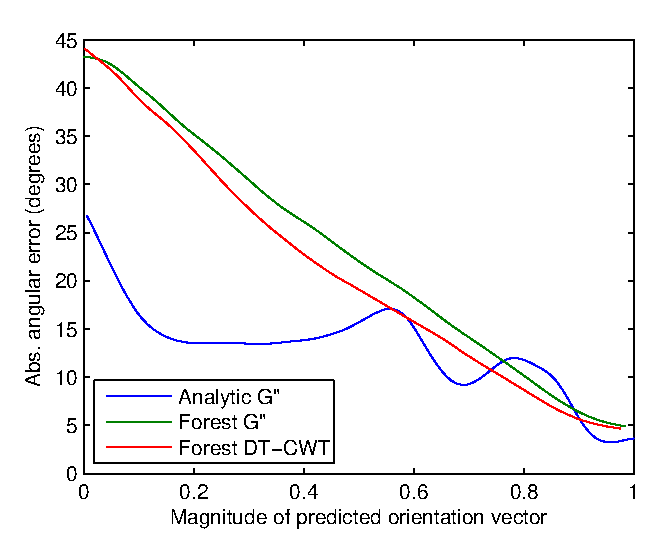
\includegraphics[width=\figwidth]{\figpath/retina/response_vs_error_ret} \\
(c) & (d)\\
\noalign{\smallskip}
\end{tabular}
%
\caption{Orientation estimation results for selected methods over pixels along the centre of the vessel: (a) Cumulative frequency of angular error; (b) Kernel estimate of mean error with respect to line thickness; (c) Kernel estimate of mean error with respect to line contrast; (d) Kernel estimate of mean error with respect to predicted orientation magnitude (for the analytic Gaussian, the absolute response scaled between 0 and 1 at the maximal angles is used).}
\label{f:retina_graphs}
\end{figure}
%
These results show that orientation was consistently estimated more accurately by regression compared to the analytic method, with particular improvement seen in faint narrow vessels. Overall, combining \dtcwt{} features with Random Forest regression was most successful with the \dtcwt{} in particular benefiting from the improvement of Random Forests over simple linear regression (\tref{t:retinopathy})

We also investigated the variation of mean angular error with respect to the magnitude of the orientation vector predicted by the regression forests (\fref{f:retina_graphs}d). The consistent reduction in angular error with increasing magnitude for all feature types confirms that this is indeed a measure of confidence in the forest prediction, whilst the same cannot be said of the magnitude of the analytic response.

Moreover, careful examination shows that while orientation magnitude is generally high at vessels (as a classifier it achieves $A_z = 0.901$) it is lower at bifurcations and crossings where orientation is not well defined, and thus provides information in addition to the classification probabilities. For example, where angular measurements are of direct interest (\eg~vessel tortuosity~\cite{Hart_etal_IJMI99}) the segmentation may suggest which pixels to include in the analysis with orientation confidence weighting the inputs. Thus the orientation confidence could sensibly down-weight the contribution of points where orientation is ill-defined even though vessel probability may be high.

Alternatively, in further processing of vessel probabilities such as using a tracking algorithm to group connected pixels, the orientation confidence can be used to control the spread of potential paths, with a narrow focus along vessel centres and a wide spread at bifurcations where the paths necessarily diverge.


\section{Conclusions}
\label{s:conclusions}
Combining suitable filters with Random Forests produces vessel segmentation that matches the state of the art without application specific post-processing as used in rival methods (and that we would expect to improve results further). Moreover, we have shown that regressing orientation estimates using similar machinery is more accurate than relying on analytical estimations. Most promisingly, the improvement in orientation estimation is greatest for particularly challenging structures such as thin, low-contrast vessels. As a further advantage of regressing with random forests, we propose that both the predicted orientation \emph{and} its associated magnitude may be useful features in further processing. Though demonstrated on retinograms, our methods are generally applicable to linear structures in any images where ground truth is available.

%\end{document}

\bibliographystyle{splncs}
\bibliography{./bib/_aliases,./bib/mobio,./bib/mammography,./bib/ml,./bib/local}

\end{document}
